

\begin{frame}{Responses}
    \begin{columns}
        \begin{column}{0.5\textwidth}
            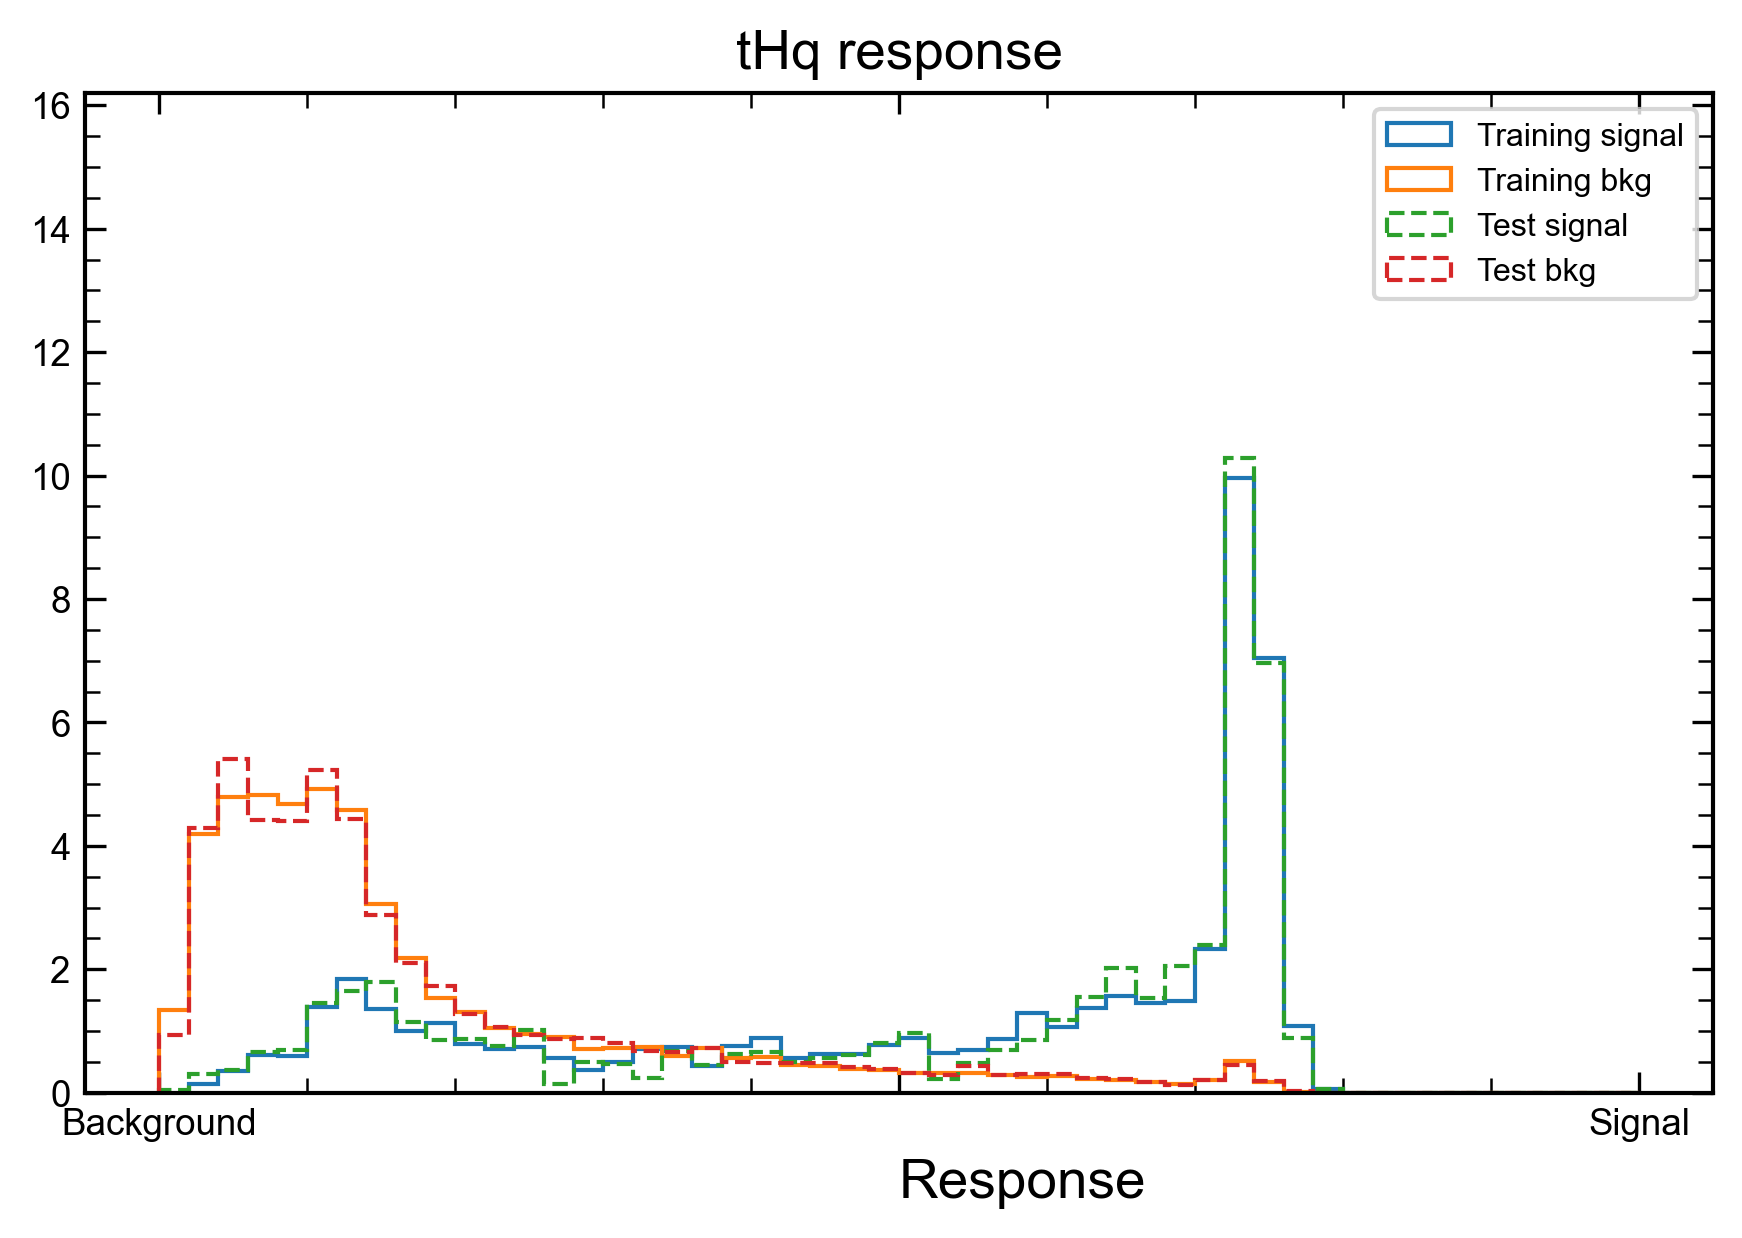
\includegraphics[width=0.8\textwidth]{response_lephad}
            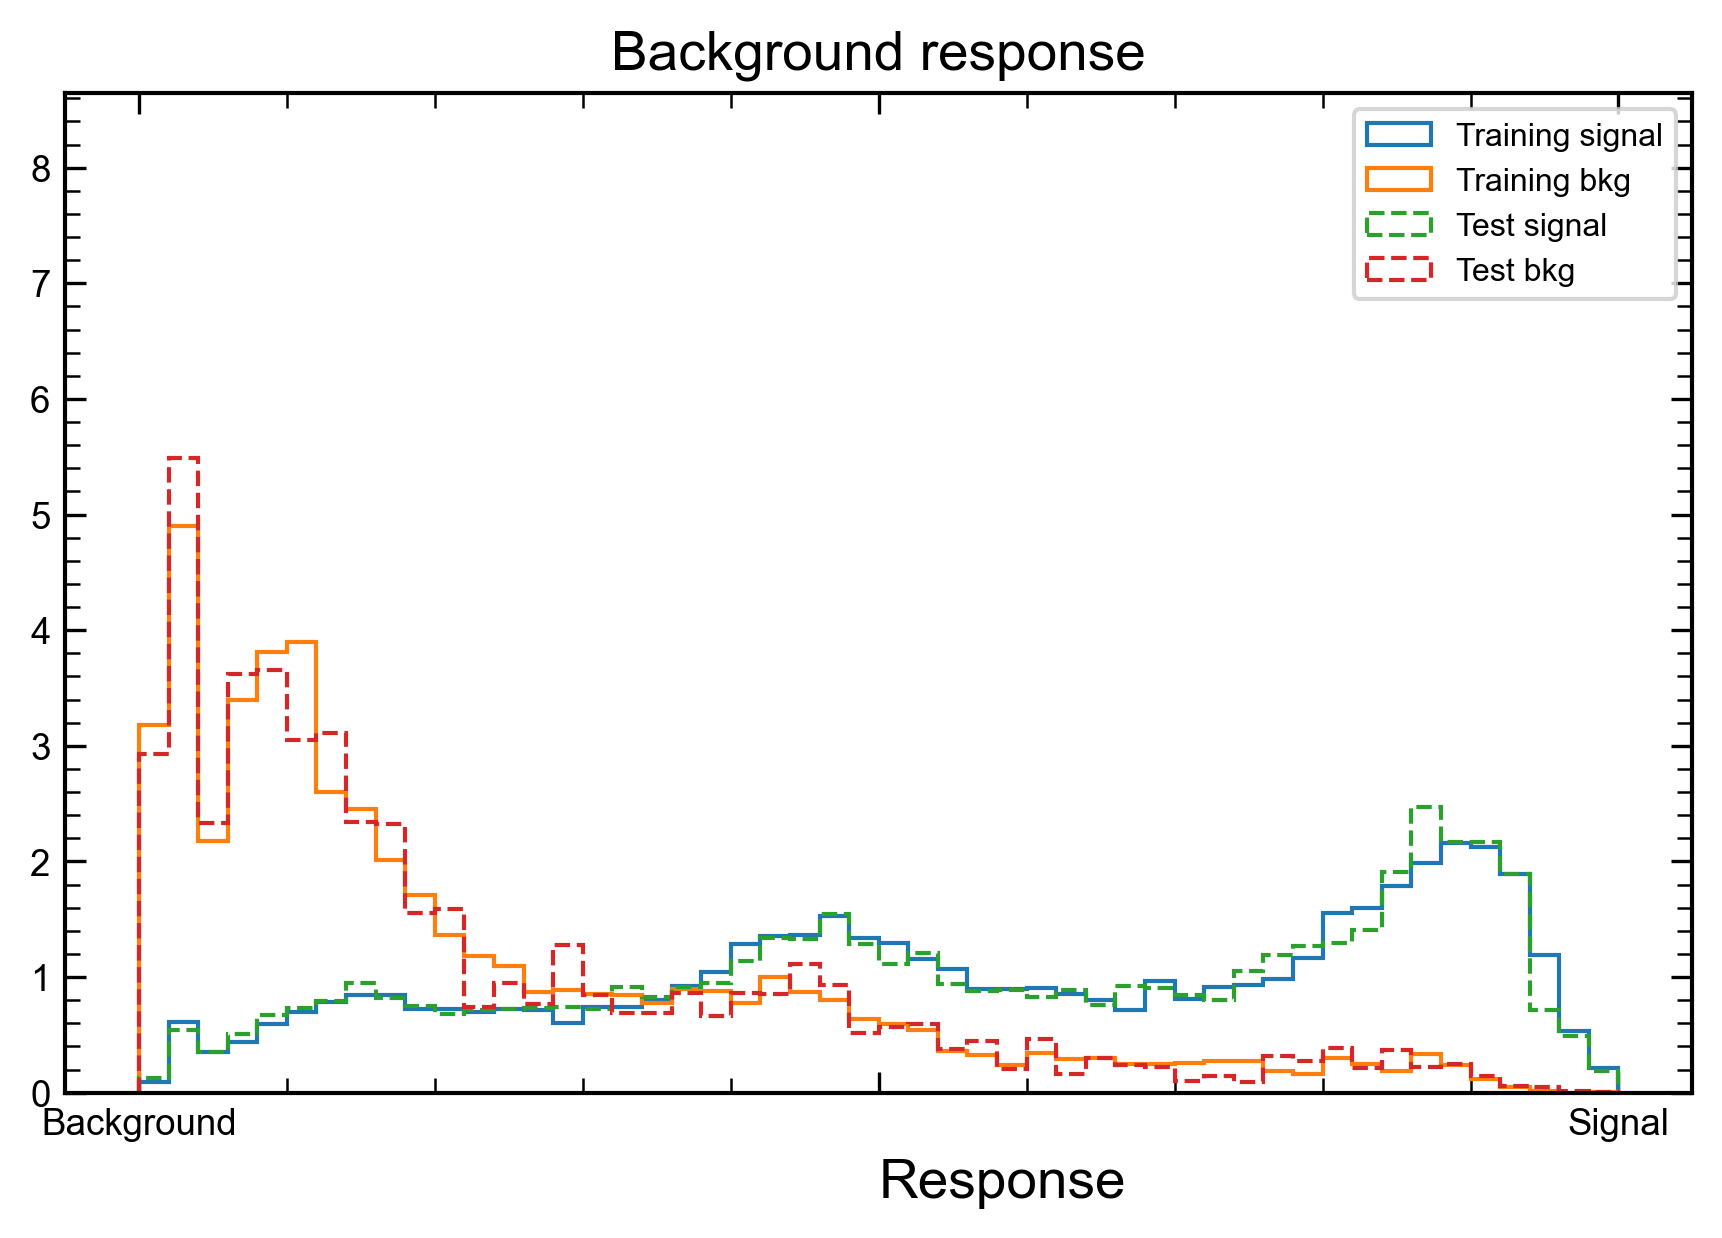
\includegraphics[width=0.8\textwidth]{bkg_lephad}
        \end{column}
        \begin{column}{0.5\textwidth}
            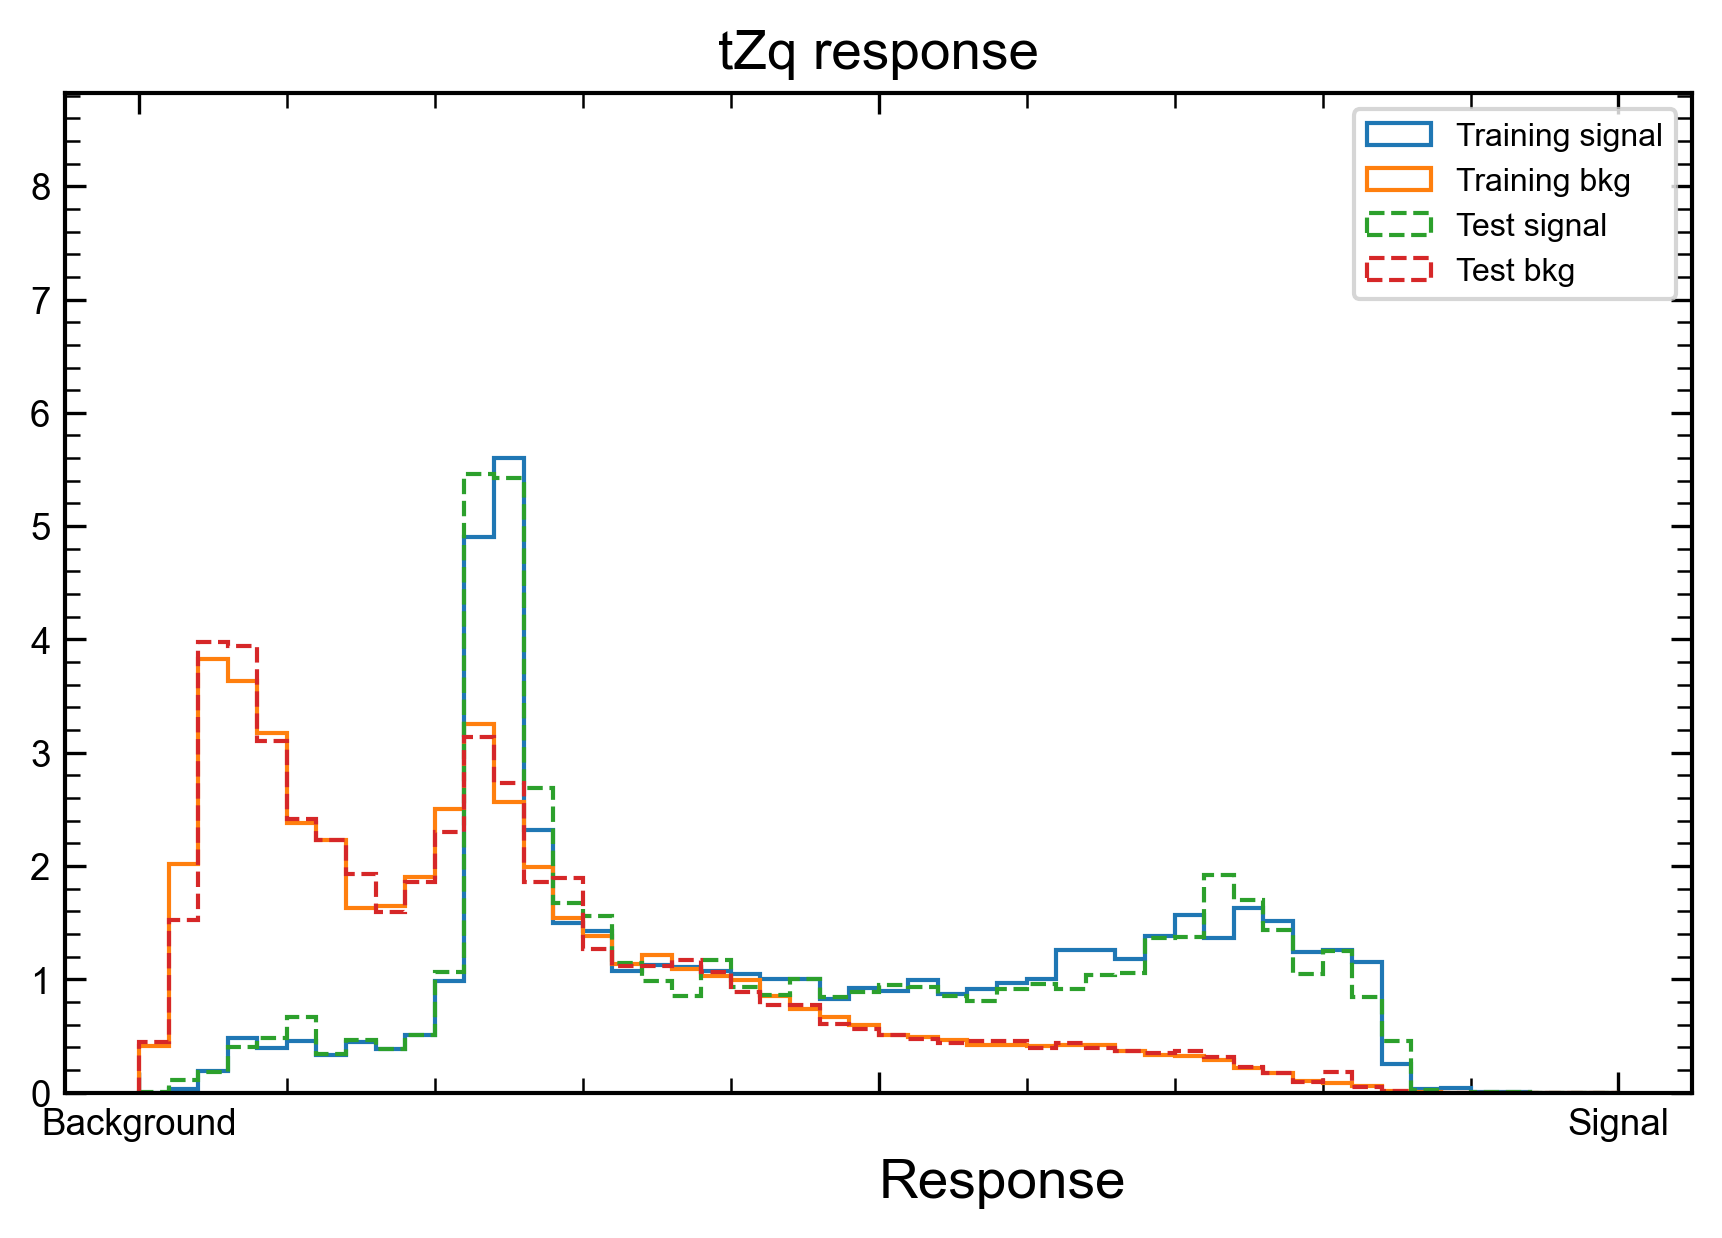
\includegraphics[width=0.8\textwidth]{tZq_lephad}
            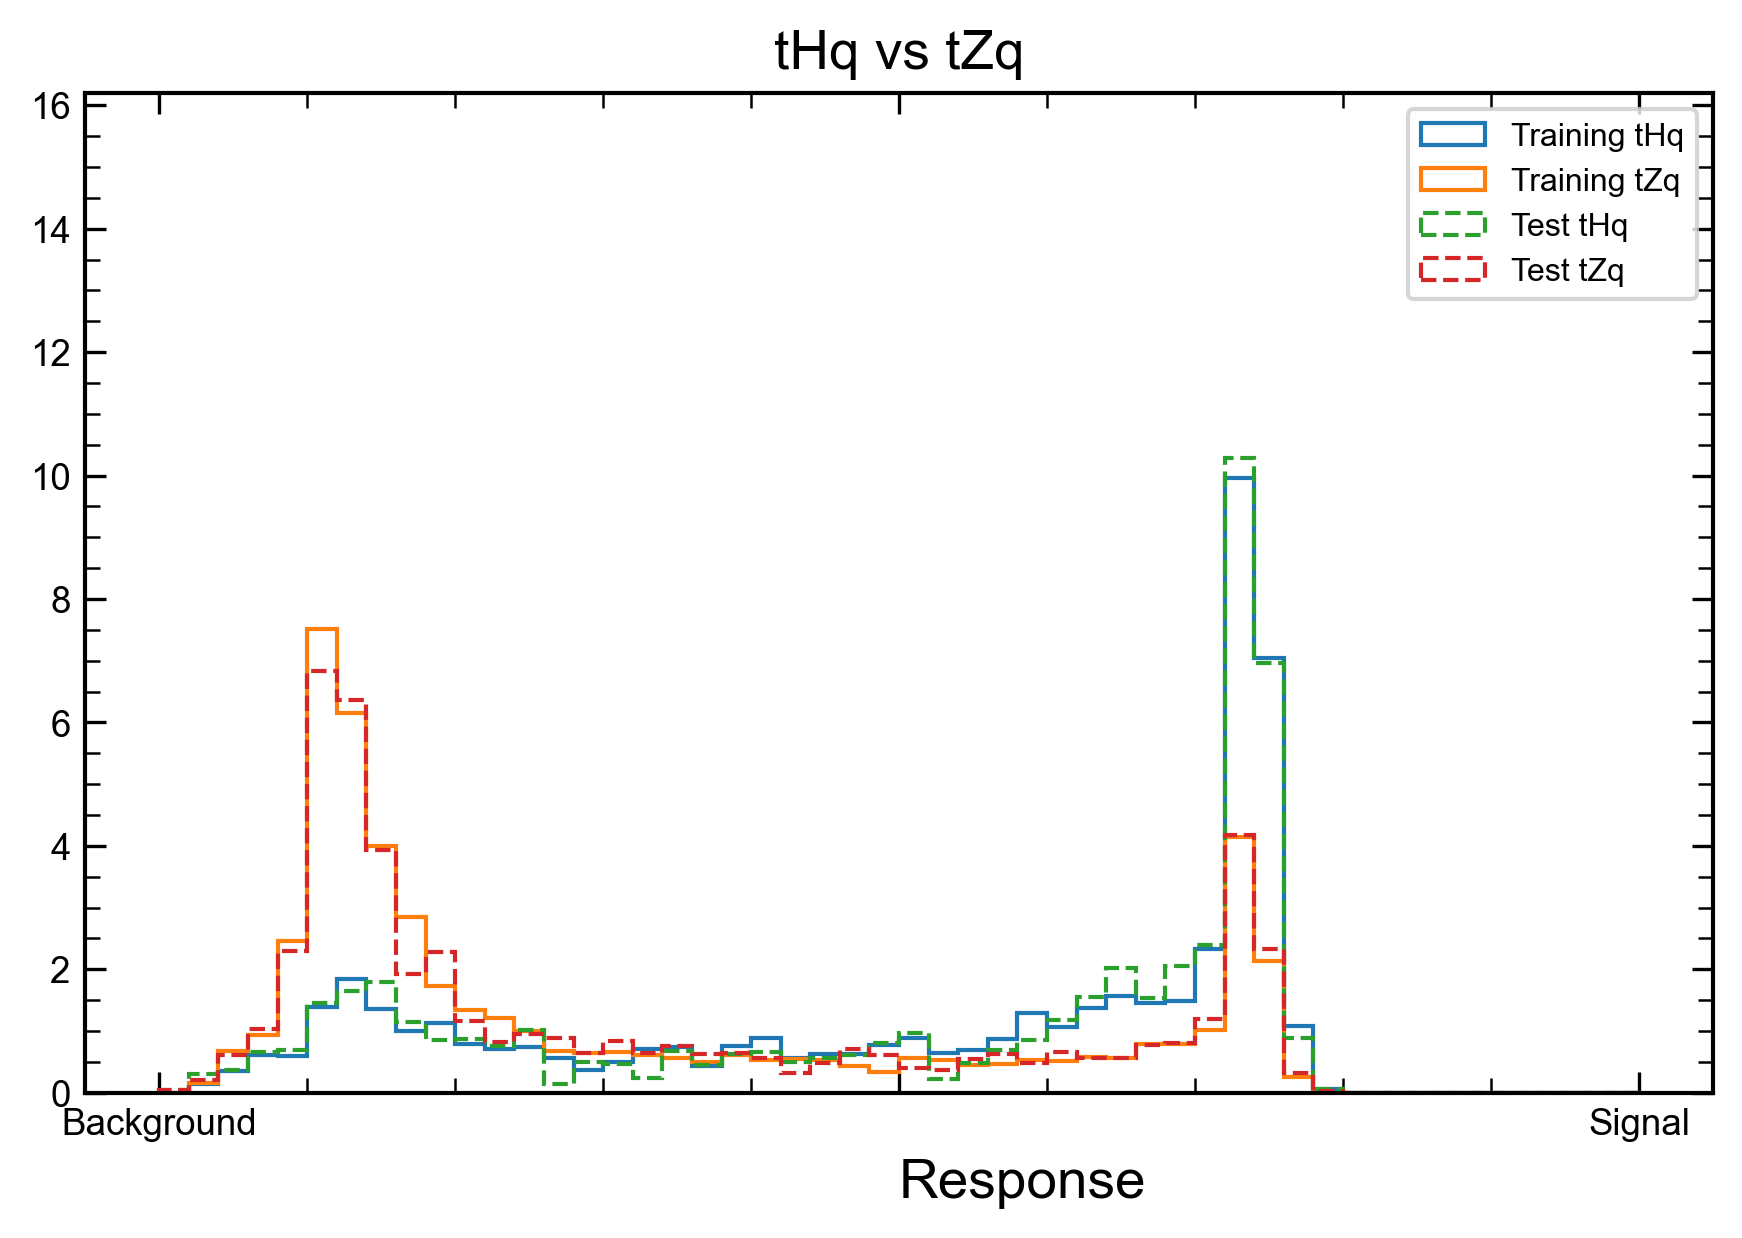
\includegraphics[width=0.8\textwidth]{comparison_lephad}
        \end{column}
    \end{columns}
\end{frame}

\begin{frame}{Yields}
    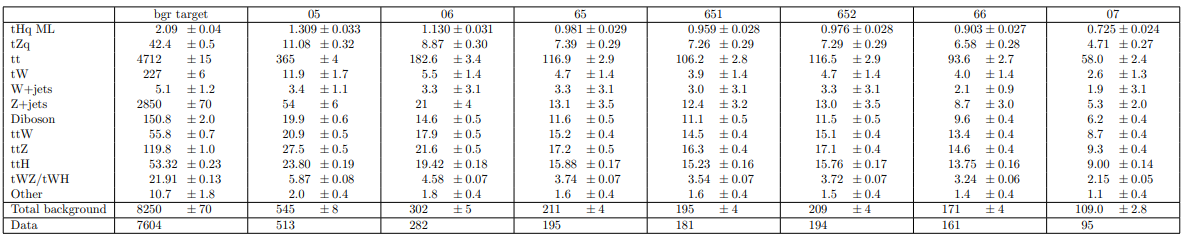
\includegraphics[width=\textwidth]{yields}
\end{frame}

\begin{frame}{S over B}
    \begin{columns}
        \begin{column}{0.5\textwidth}
            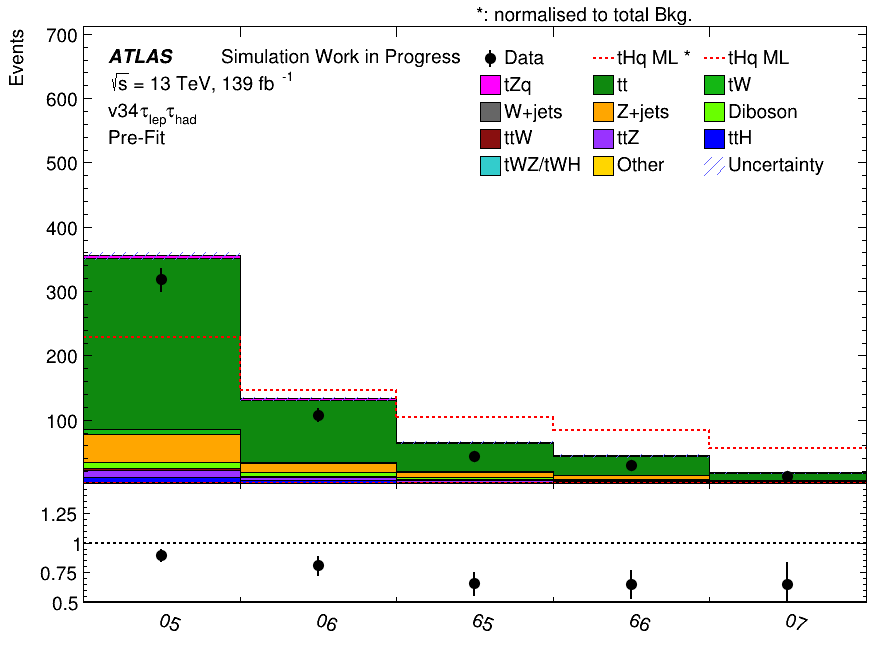
\includegraphics[width=0.8\textwidth]{Summary}
        \end{column}
        \begin{column}{0.5\textwidth}
            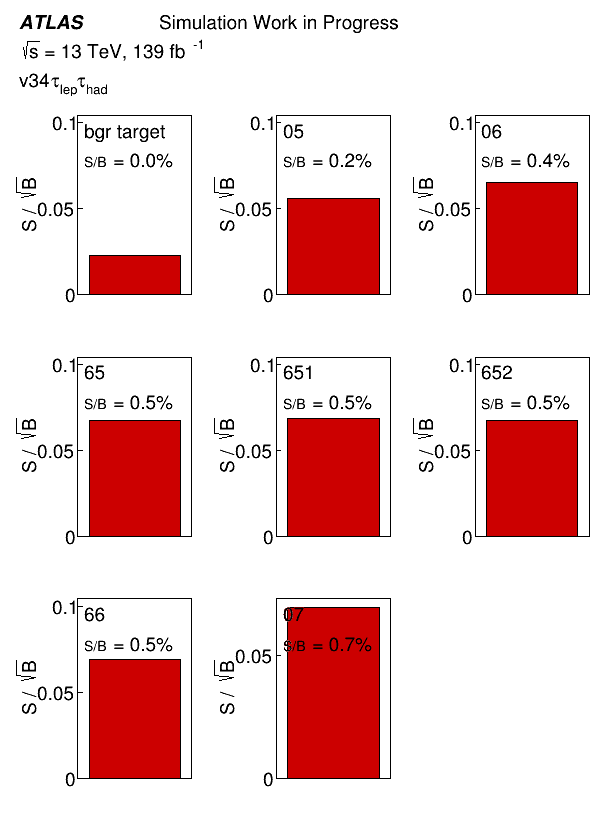
\includegraphics[width=0.8\textwidth]{soverb}
        \end{column}
    \end{columns}
\end{frame}

\begin{frame}{Summary}
    \begin{itemize}
        \item Every tool necessary to fit with the NN output is in place and tested 
        \item The model shows good stability and tests for negative weights setups hold
        \item Additionally, feature behaviour with respect wo weight sign was investigated
        \item Test fits created for lephad (and hadhad)
        \item Variable ranking planned, only needed for documentation
        \item Improved performance expected from combining categorical likelihhods, simple 2D cut not enough.
    \end{itemize}
\end{frame}

